\documentclass[letterpaper]{article}

\usepackage[spanish]{babel}				%idioma fuente
\usepackage[utf8]{inputenc}				%acentos
\usepackage{amsmath}					%matemáticas
\usepackage{amsfonts} 					%fuente de matemáticas
\usepackage{amssymb}
\usepackage{booktabs}					%Incluir tablas
\usepackage{graphicx}					%Incluir impagenes
\usepackage{fancyhdr} 					%encabezados
\usepackage[lofdepth, lotdepth]{subfig} %colocar varias figuras
\usepackage{listings}					%pegar códigos de matlab y se vean presentables
\usepackage{placeins}
\usepackage{float}
\usepackage[left=2.54cm,right=2.54cm,top=2.54cm,bottom=2.54cm]{geometry}
\lstset{language=Scilab, breaklines=true, basicstyle=\footnotesize}
\lstset{numbers=left, numberstyle=\tiny, stepnumber=1, numbersep=-8pt}

	%------------------------ENCABEZADO Y PIE DE PÁGINA-------------------%
\lhead{Control I}
\rhead{Analysis of a First Order System}
\lfoot{Depto. de Ingeniería Electrónica}
\cfoot{\thepage\ de \pageref{LastPage}}
\rfoot{Instituto Tecnológico de Morelia}

\title{Instituto Tecnológico de Morelia\\
		{\small DIVISIÓN DE ESTUDIOS PROFESIONALES
		\\DEPARTAMENTO DE INGENIERÍA ELECTRÓNICA\\CONTROL I\\\vspace*{0.2in} REPORTE DE PRÁCTICA 1}\\ "Analysis of a First Order System"}

\author{
	\textbf{EQUIPO "Mendoza - Ramírez"} \\\\
	\textbf{INTEGRANTES:}\\
	\\ Mendoza Sánchez Alainn Ezzequiel.	14121100 
	\\ Ramírez Espinosa 	Rodrigo.	14121137 \\\\ 
	\textbf{Semestre:} \\\\ Agosto-diciembre 2017\\\\ 
	\textbf{Profesor:} \\\\ M.C. Gerardo Marx Chávez Campos \\\\ 
	\textbf{Fecha de entrega:} 27 de Octubre de 2017}
\date{}

\begin{document}
		\begin{figure}[t]
		\centering
		
\includegraphics[scale=0.7]{Header}
	\end{figure}
	\pagenumbering{gobble}
	\maketitle
	\pagebreak
	\pagenumbering{arabic}
	\newpage
	\section{Introducción.}
	El principal objetivo principal de esta práctica, es demostrar por medio del análisis un sistema de control hidráulico para un tanque de almacenamiento de agua, el cual posee un un flujo de entrada y un flujo de salida, este última controlado por una llave para modular el flujo de salida. Cabe mencionar que el nivel de agua en el tanque depende tanto de la cantidad del flujo de entrada como también del orificio de salida determinado por la llave.\\\\
	Una vez analizado esto, se tuvo que obtener una ecuación del balance de energía del sistema hidráulico en cuestión, y posteriormente se procedió a realizar una analogía de la ecuación mediante un circuito eléctrico, ya que, el flujo de agua representa el flujo de corriente en el circuito.\\\\
	Durante las sesiones de laboratorio, el profesor nos proporcionó una función de transferencia en el Software \textbf{Scilab}, para de ahí partir graficando la respuesta del sistema hidráulico. Posteriormente tuvimos que realizar un código que nos diera los mismos resultados que el código proporcionado por el profesor, modificando el código para que resolviera la función de transferencia por medio de fracciones parciales y después aplicara ta Transformada inversa de Laplace, para así obtener la respuesta en función del tiempo y, dándole valores a las variables de las ecuaciones, graficar tres condiciones del sistema: cuando la entrada sea \textbf{igual} a la salida, cuando la entrada sea \textbf{menor} a la salida y cuando la salida sea \textbf{mayor} a la entrada.
	
	\newpage
	\section{Metodología.}
	Como ya se sabe, la función de transferencia está definida como:
	\begin{equation}
	H(s)=\frac{Y(s)}{X(s)}
	\end{equation}
	De manera que si despejamos la salida $ Y(s) $
	\begin{equation}
	Y(s)=H(s)+X(s)
	\end{equation}
	Se puede considerar que la entrada $ X(s) $ es una respuesta de escalón unitario, por lo que:
	\begin{equation}
	Y(s)=\frac{1}{s} * X(s)
	\end{equation}	
	En base a lo anterior, se puede considerar una función de transferencia genérica
	\begin{equation}
	H(s)=\frac{bs+c}{s+a}
	\end{equation}
	En donde $ a $, $ b $ y $ c $ son números reales. Despejando la salida $ Y(s) $ y con la respuesta de escalón unitario se tiene
	\begin{equation}
	Y(s)=\frac{1}{s} * \frac{bs+c}{s+a}
	\end{equation}
	Y para poder resolver la ecuación $ (5) $ utilizamos el método de fracciones parciales, quedando la función de la siguiente manera:
	\begin{equation}
	Y(s)=\frac{A}{s} * \frac{B}{s+a}
	\end{equation}
	Al resolver la ecuación $ (6) $, obtuvimos los valores de $ A $ y $ B $ en términos de $ a $, $ b $ y $ c $, donde:
	\begin{equation}
	A=\frac{c}{a}\hspace{0.5cm}y\hspace{0.5cm}B=b-\frac{c}{a}
	\end{equation}
	Al sustituir $ A $ y $ B $ en $ (6) $, tenemos:
	\begin{equation}
	Y(s)=\frac{c}{a*s} * \frac{b-\frac{c}{a}}{s+a}
	\end{equation}
	La ecuación $ (8) $ nos mostrará directamente la función de transferencia de salida, por lo que, obteniendo la transformada inversa de $ (8) $, tendremos la respuesta de la salida con respecto al tiempo:
	\begin{equation}
	Y(t)=\frac{c}{a}*(b-\frac{c}{a})*e^{-at}
	\end{equation}
	
	\newpage
	\textbf{Ejemplo:}
	La respuesta de escalón unitario para el siguiente sistema es:	
	\begin{figure}[h!]
		\centering
		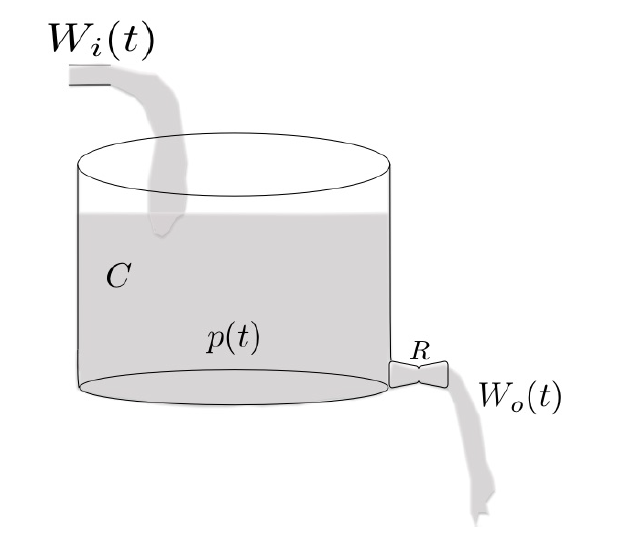
\includegraphics[scale=.75]{tank}
		\caption{Esquema de sistema hidráulico.}
	\end{figure}
	\FloatBarrier
	Se sabe que la energía de entrada más la energía generada es igual a la energía acumulada más la energía de salida, de acuerdo a la ecuación de Bernoulli, tal definición se puede presentar mediante la siguiente fórmula:
	\begin{equation}
	\sum E_{in} + \sum E_{Gen} = \sum E_{out} + \sum E_{acu}
	\end{equation}
	Podemos despreciar el valor de la energía generada, ya que no se acumula agua de manera automática dentro del contenedor. De manera que:
	\begin{equation}
	\sum E_{in} = \sum E_{out} + \sum E_{acu}
	\end{equation}
	 La energía de entrada está dada por el flujo de entrada $ W_{in} $, la energía de salida está dada por $ W_o $ y la energía acumulada está dada por $ A=\frac {dp(t)}{dt} $, entonces:
	 \begin{equation}
	 W_{in}=W_o + A\frac{dp(t)}{dt}
	 \end{equation} 
	 Pero, sabemos que $ W_o $ es igual al área del orificio de salida por $ p(h) $ entre la resistencia $ R $ del flujo:
	 \begin{equation}
	 W_{in}(t)=\frac{rg*p(t)}{R}+A\frac{dp(t)}{dt}
	 \end{equation}
	 
	 \newpage
	 Que también puede ser representada por medio de una analogía de corrientes del circuito eléctrico de la \textbf{Figura 2}, en donde $ Re =\frac{R}{rg}$:
	 \begin{equation}
	 W_{in}(t)=\frac{p(t)}{Re}+Ce\frac{dp(t)}{dt}
	 \end{equation}
	 Que es igual a:
	 \begin{figure}[h!]
	 	\centering
	 	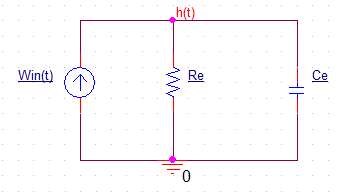
\includegraphics[scale=.9]{cir}
	 	\caption{Analogía del esquema hidráulico a un circuito eléctrico analizado por corrientes.}
	 \end{figure}
 	\FloatBarrier
 	Aplicando la transformada de Laplace a la ecuación $ (14) $ tenemos:
 	\begin{equation}
 	W_{in}(s)=\frac{p(s)}{Re}+Cep(s)+p(0)
 	\end{equation}
 	En donde $ p(o) = 0$, ya que no hay un valor inicial. Para obtener la función de transferencia, factorizamos $ p(s) $ y obtenemos $ \frac{p(s)}{W_{in}(s)}=H(s) $
 	\begin{equation}
 	H(s)=\frac{Re}{1+ReCes}
 	\end{equation}
 	
 	\newpage
 	\section{Resultados.}
 	El siguiente código fue el empleado en la solución del ejemplo anterior en base a la función de transferencia genérica de la ecuación $ (4) $, obteniendo la función $ (8) $ introduciendo los valores numéricos de $ a $, $ b $ y $ c $ de la ecuación $ (5) $.
 	También arroja una gráfica en función de $ (t) $ de la salida.
	\begin{lstlisting}
	clear all
	clc
	s=poly(0,"s");
	disp('En base a la ecuacion:');   //Arrojar a la pantalla "En base a la ecuacion"
	disp('Ys=(1/s)*(((b*s)+c)/((s)+a))');   //Ecuacion para identificar a, b y c
	a=input('Ingrese el numero correspondiente a:');  //Introducir valor a
	b=input('Ingrese el numero correspondiente b:');  //Introducir valor b
	c=input('Ingrese el numero correspondiente c:');  //Introducir valor c
	FT=(c/(a*%s))+((b-(c/a))/((%s)+a));    //Funcion de transferencia para Y(s)
	disp('Y(s) simplificado es:');  //Simplificado de la funcion de transferencia
	disp(FT);   //Mostrar en pantalla la funcion de transferencia simplificada
	A=(c/(a*%s));   //Guardar en A la primera fraccion parcial
	B=((b-(c/a))/((%s)+a));   //Guardar en B la segunda fraccion parcial
	disp('Y(s) es:');   //Mostrar en pantalla "Y(s) es:"
	Ys=[A B];   //Guardar en un vector A y B
	disp(Ys);   //Mostrar en un vector Y(s)
	t=0:0.01:20;   //t tomara valores del 0 al 20 cada 0.01 valores
	yt=(c/a)+((b-(c/a))*exp(-a*t));   //Y(t) sera la salida en funcion del tiempo
	plot(t,yt)   //Graficar yt con respecto a t
	title('Respuesta de la funcion de transferencia en el tiempo')//Titulo de la grafica
	xlabel('Tiempo t')   //Nombre del eje de las "x"
	ylabel('Y(t)')   //Nombre del eje de las "y"
	\end{lstlisting}
	El siguiente código es el código de Scilab:
	\begin{lstlisting}
	// Copyright (C) 2017 - Instituto Tecnologico de Morelia 
	// by Gerardo Marx Chavez-Campos
	// This code has been developed for educational propouses
	// the institution and author do not guarantee  the proper
	// functionality of the code.
	//
	// Date of creation: Oct 2, 2017
	s = %s // The quicker alternative to using s =
	poly (0 , 's' ) 
	// Gain and time constant
	K = 1;  
	Tau = 1; 
	simpleSys=syslin('c', K/(1+Tau*s))
	t=0:0.01:15;
	y=csim('step', t, simpleSys)
	plot(t,y)	
	\end{lstlisting}
	Cuando en el código implementado por nosotros, introducimos los valores de $ a=1 $, $ b=0 $ y $ c=1 $, obtenemos una respuesta igual al código propuesto por el profesor:
	\begin{figure}[h]
		\centering
		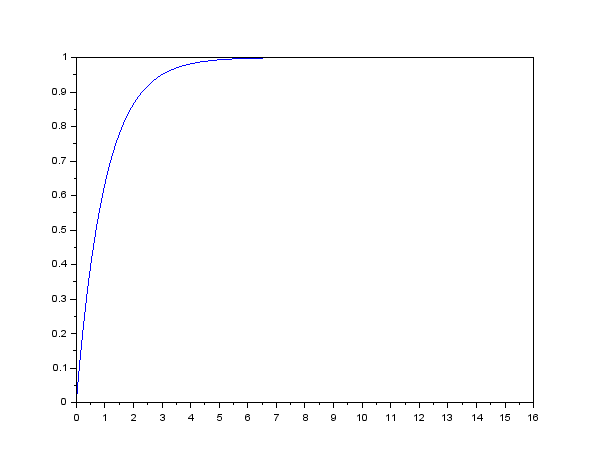
\includegraphics[scale=.7]{gra}
		\caption{Gráfica de la salida del sistema en función del tiempo con el código de Scilab proporcionado por el profesor.}
	\end{figure}
	\begin{figure}[h]
		\centering
		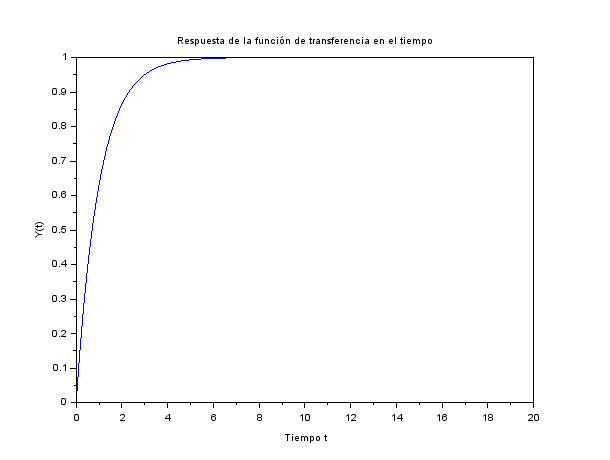
\includegraphics[scale=.7]{gra2}
		\caption{Gráfica de la salida del sistema en función del tiempo con el código de Scilab realizado por nosotros.}
	\end{figure}
	\FloatBarrier
	En el sistema hidráulico se pueden ancontrar tres casos diferentes: Cuando $ W_{in}=W_o $, cuando $ W_{in}>W_o $ y cuando $ W_{in}<W_o $.\\\\
	Para el primer caso, que es cuando $ W_{in}=W_o $, tenemos que, en el circuito de la \textbf{Figura 2} no existe capacitor, por lo que la corriente que suministra la fuente de corriente es la misma corriente que circula por la resistencia, siendo esta corriente la de $ W_o $.\\\\
	La respuesta de este sistema será de 1, debido a que la entrada y la salida son iguales, por lo que la función de transferencia o ganancia será de 1, y esto se puede obtener introduciendo los valores de $ a=1 $, $ b=1 $ y $ c=1 $ en el código realizado por nosotros.\\\\
	Con esto vemos que el segundo término se hace $ 0 $, teniendo la función lineal esperada:
	\begin{figure}[h!]
		\centering
		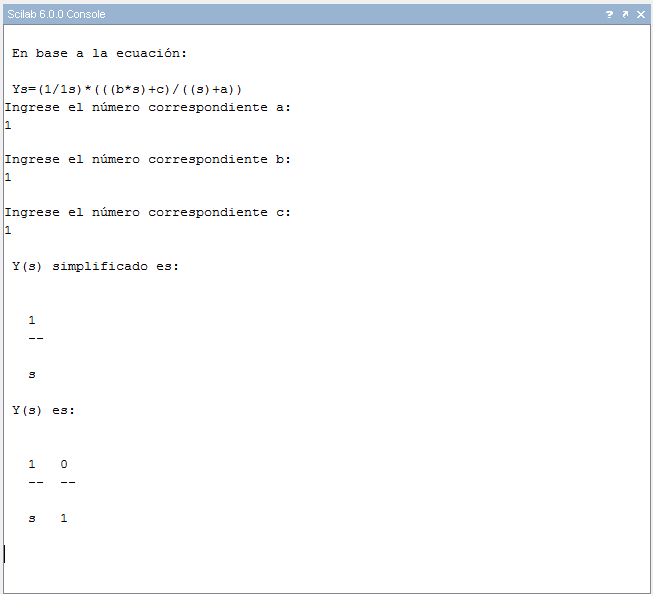
\includegraphics[scale=.6]{cod}
		\caption{Respuesta de la consola de Scilab con $ a=1 $, $ b=1 $ y $ c=1 $.}
	\end{figure}
	\FloatBarrier
	\begin{figure}[h!]
		\centering
		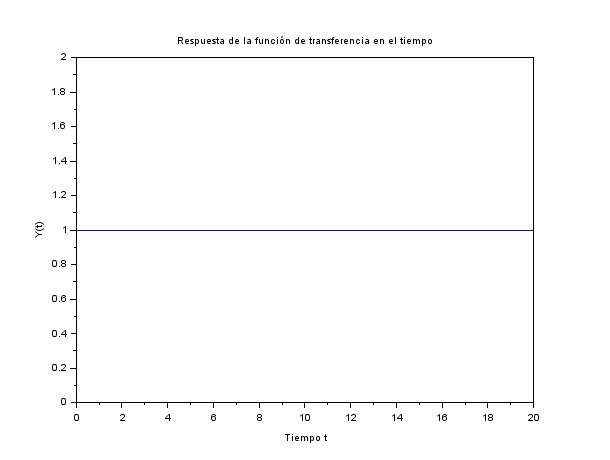
\includegraphics[scale=.7]{gra1}
		\caption{Gráfica de la función de salida cuando $ W{in}=W_o $.}
	\end{figure}
	\FloatBarrier
	Para el segundo caso, que es cuando \textbf{$ W_in>W_o $}, podemos ver en base al circuito de la \textbf{figura 2} que toda la corriente de entrada ($ W_in $) debe ser mucho mayor a la corriente de la resistencia ($ W_o $). Con esto podemos concluir que la resistencia tiene que tender al infinito, de manera que la mayoría de la corriente tienda a pasar por el capacitor.
	Entonces, en base a la ecuación $ (14) $, si $ Re $ tiende al infinito, $ W_o $ tenderá a $ 0 $. Si sustituimos $ Re=1000Re $ en la ecuación $ (14) $, tenemos:
	\begin{equation}
	W_{in}(t)=\frac{p(t)}{1000*Re}+Ce\frac{dp(t)}{dt}	
	\end{equation}
	Transformando a Laplace:
	\begin{equation}
	W_{in}(s)=0.001*W_o(s)+Cep(s)s
	\end{equation}
	Si multiplicamos $ Cep(s) $ por $ \frac{Re}{Re} $, tendremos:
	\begin{equation}
	W_{in}(s)=0.001*W_o(s)+Cep(s)s(\frac{Re}{Re})
	\end{equation}
	\begin{equation}
	W_{in}(s)=0.001*W_o(s)ReCes
	\end{equation}
	\begin{equation}
	\frac{W_{in}(s)}{W_o(s)}=0.001+ReCes
	\end{equation}
	\begin{equation}
	\frac{W_o(s)}{W_{in}(s)}=\frac{1}{(0.001+ReCep(s)s)}
	\end{equation}
	Al multiplicar todo por $ \frac{\frac{1}{ReCe}}{\frac{1}{ReCe}} $ para dejar a $ s $ sola, tenemos:
	\begin{equation}
	\frac{W_o(s)}{W_{in}(s)}=\frac{\frac{1}{ReCe}}{(\frac{0.001}{ReCe}+s)}
	\end{equation}
	La ecuación $ (23) $ se parece al segundo término de la ecuación $ (8) $, por lo que $ a $ tiende a $ 0 $ para $ W_{in}>W_o $. Introduciendo estos valores al programa que creamos en Scilab, obtuvimos:
	\begin{figure}[h]
		\centering
		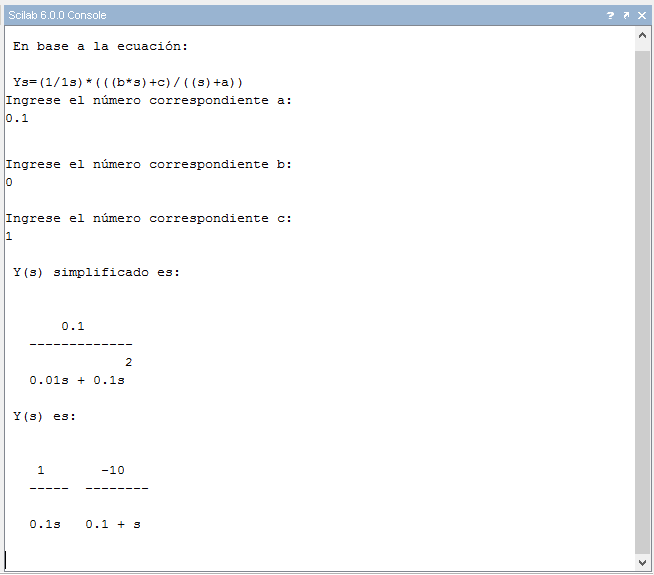
\includegraphics[scale=.6]{cod2}
		\caption{Respuesta de la consola de Scilab con $ a=0.1 $, $ b=0 $ (para que inicie en $ 0 $) y $ c=1 $.}
	\end{figure}
	\begin{figure}[h]
		\centering
		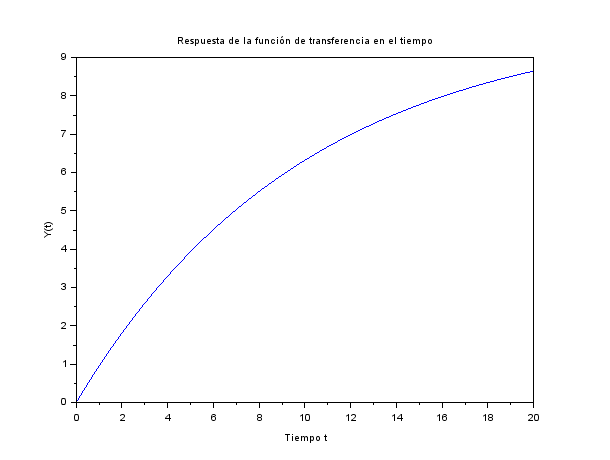
\includegraphics[scale=.7]{gra3}
		\caption{Gráfica de la función de salida cuando $ W_{in}>W_o $}
	\end{figure}
	\FloatBarrier
	El comportamiento de la \textbf{figura 8} se debe a que el flujo de entrada es mayor al de la salida, por lo que el contenedor está en constante llenado.\\\\	
	Para el último caso, es decir, cuando $ W_{in}<W_o $, se hace el mismo procedimiento del caso cuando $ W_{in}>W_o $, pero haciendo que el valor de $ a $ sea contrario, en otras palabras, $ a $ ahora tenderá al infinito.
	\begin{figure}[h]
		\centering
		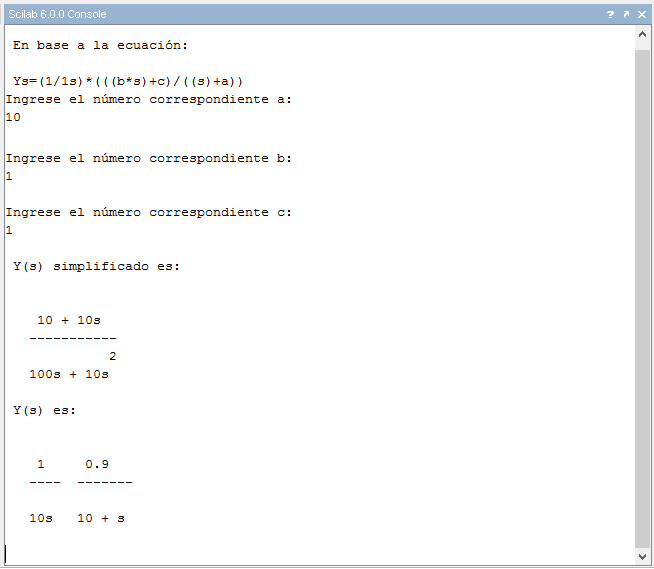
\includegraphics[scale=.5]{cod3}
		\caption{Respuesta de la consola de Scilab con $ a=10 $, $ b=1 $ y $ c=1 $.}
	\end{figure}
	\FloatBarrier
	\begin{figure}[h]
		\centering
		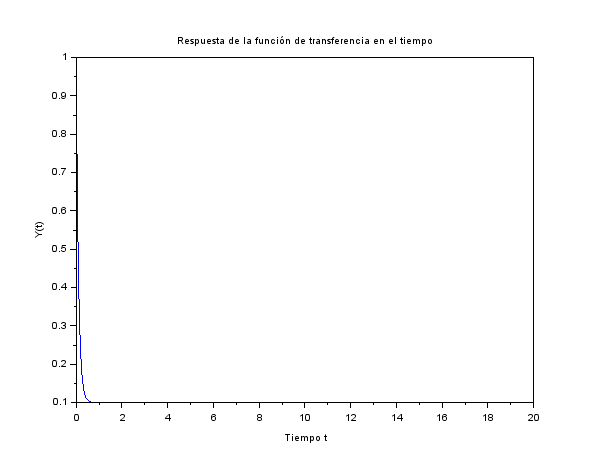
\includegraphics[scale=.65]{gra4}
		\caption{Gráfica de la función de salida cuando $ W_{in}<W_o $.}
	\end{figure}
	\FloatBarrier
	El comportamiento de la \textbf{Figura 10} es coherente, ya que cuando el área del orificio de la salida es más grande que el de la entrada, no habrá almacenamiento de agua dentro del contenedor, por lo que será $ 0 $.
		
	\newpage
	\section{Conclusiones.}
	
	\textbf{Mendoza Sánchez Alainn Ezzequiel (14121100):}\\\\
		Puedo concluir que en esta práctica nos demuestra que lo visto en clase y se emplea en la práctica resulta exitoso, ya que pudimos observar que se puede hacer una representación de la respuesta de un sistema, por medio de la función de transferencia. En clase lo vimos como representaciones mecánicas, pero en la práctica lo empleamos como representación hidráulica, obteniendo la respuesta del sistema en tres diferentes casos, los cuales se pudieron llevar a cabo al emplear la respuesta del escalón unitario, enconjunto con una función de transferencia genérica.\\
	
	\textbf{Ramírez Espinosa Rodrigo (14121137):}\\\\
		Con esta práctica realizada se pudo observar que, en efecto, la función de transferencia es un modelo matemático que representa la respuesta de un sistema. Esto se pudo observar en el ejemplo hidráulico, ya que por medio de la respuesta en el escalón unitario y la función de transferencia genérica se pudo obtener la respuesta de dicho sistema hidráulico en sus tres casos analizados.

\end{document}